\documentclass{llncs}
\usepackage{graphicx}
\usepackage{hyperref}
% section symbol
\usepackage{cleveref}

%\renewcommand\UrlFont{\color{blue}\rmfamily}
%Jorge Altamirano-Astorga, Edgar Francisco Román-Rangel
%Ita-Andehui Santiago-Castillejos, 
%Luz Aurora Hernández-Martínez
    
\begin{document}

    \title{Indoor Air Pollution Forecasting using Deep Neural Networks}
    
    \author{Jorge Altamirano-Astorga \and
        Ita-Andehui Santiago-Castillejos \and
        Luz Hernández-Martínez \and
        Edgar Roman-Rangel}
    \authorrunning{J. Altamirano-Astorga et al.}
    \institute{
        Instituto Tecnológico Autónomo de México, Mexico City, Mexico
        \url{https://philwebsurfer.github.io/dlfinal/}
        \email{\{jaltami9,isantia2,lhern123,edgar.roman\}@itam.mx} 
    }
    
    \maketitle
 
    \begin{abstract}
        Atmospheric pollutants have negative incidence in the life of 
        people and people tend to stay indoor, specially during COVID-19 
        pandemic. Using deep learning techniques leveraged by the large 
        processing capabilities of powerful cloud computing environments
        to compare forecasting capabilities of Artificial Neural Networks
        that model time series data such as indoor air quality using 
        a home sensor together with outdoor air quality information from
        public and private data sources. Comparing different ANN and
        automatic hyperparameter tuning can be relevant for further research
        for this type of datasets.
        \keywords{Deep Learning \and
            Artificial Neural Networks \and
            Indoor Air Quality Forecasting \and
            Cloud Computing
        }
    \end{abstract}

    \hypertarget{introduction}{%
\section{Introduction}\label{introduction}}


Monitoring of air quality and the forecast of air pollution are both
paramount for many daily activities \cite{patni}, as air quality has 
direct impact on
human health, agriculture, and the environment in general. Moreover, it
is directly related to global warming and climate change \cite{airpollution}.

%As it has been the case with other Pattern Recognition applications,
%Deep Learning has shown improved success also in the forecast of air
%quality with respect to traditional methods like ARIMA or exponential
%smoothing (ES) {[}cite{]}.

Usually, air quality systems focus on monitoring specific components of outdoors atmospheric pollutants,
including $NO_{2}$, $NO_{3}$, $NO_{x}$, $O_{2}$, $CO_{2}$, $PM_{10}$, 
$PM_{2.5}$, and $IAQ$ index, using public monitoring stations that report their concentrations
either daily, hourly, or by the minute \cite{bme680}. However, some times
these reports might be inaccurate, noisy, or simply not provided by the
official sources during specific periods \cite{nom156}, which might have
negative consequences in human health, specially in large metropolitan
areas. Moreover, tracking indoors air quality seems thus far a 
neglected research area.

To face the potential lack of public information, as well as to contribute to the monitoring of indoors air quality, we propose the use of
affordable indoors devices, that report air quality every few seconds,
and that can be installed inside apartments. We evaluate the predictive
performance of different deep neural network-based
approaches in the task of predicting air quality IAQ. Namely, we compare
the performance of the multi-layer perceptron (MLP), convolutional neural
networks (CNN), and the long short-term memory (LSTM). Our results show
that it is possible to obtain an air quality monitoring system that is
affordable and reliable for domestic usage.

The rest of this paper is organized as follows. Section 2 comments on
previous work using deep learning techniques for air quality prediction.
Section 3 provides details on the data acquired with the indoors device.
Section 4 explains the different architectures evaluated for the task of
air quality forecast. Section 5 presents our results, and section 6 our
conclusions.

    \hypertarget{related-work}{%
\section{Related Work}\label{related-work}}

There are some underlying reproductions that use models of neural
systems from the perspective of their understanding of how neural
networks work. Among other things, we find that some authors work with
artificial neural nets based on perceptron-based architecture 
\cite{ghazali}, unlike this research who tries different architectures, 
mainly based on LSTM. In addition to this, we try with different 
time windows and other hyperparameter tuning in order to find the
one that best predicts the air quality index.

Some researchers have proposed a framework or a system to monitor IAQ
using wireless sensor networks, while others, 
we concluded, have incorporated index calculation to determine the 
IAQ level. Also, we compare our data with data from other sources
such as OpenWeatherMap \cite{openweather} and Mexico City Air Quality
\cite{sinaica,sedema}.

It is common, based on the scope of our investigations, that IAQ
monitoring Artificial Neural Networks (ANNs) are used to predict 
or forecast the value of air quality 
or the value of air pollution. In this manner, this project differs from
previous research because we use a wide variety of architectures and
expand processing capacity with Vertex Google. The functionality of this
system and the methodology of this project are explained in the next
section.

We didn't find any outstanding results for predicting any weather or
pollution in any of the papers cited. So, it is natural to build and
improve upon these weaknesses and address them.

In the paper of Abdullah \cite{abdullah} the authors make special emphasis
on the complexity and non-linear associations between air quality,
meteorological, and traffic variables. And the limitation of traditional
machine learning methods. They also had the idea of update an ANN
weights with genetic algorithms and named it optimized ANN (OANN). The
data includes 16 hours of daily information from 2014 to 2016, it came
from the Ministry of Works, Malaysia, while the air pollution and
meteorological datasets are collected from the Department of Environment
(DOE), Malaysia. These data were used to predict the concentration of
$CO$, $NO$, $NO_{2}$, and $NO_{x}$. The models included are ANN, RF, Decision Trees,
and the metrics used to measure their performance were: MAE and MSE for
all four pollutants.

The objective of the work of Cakir \cite{cakir}, 2020 was to compare the
performance of the ANN vs multiple linear regression, associating the
weather condition with some ambient air measures. The data correspond to
the average hourly concentrations of the particles during the years
2012-2015. The authors make predictions of PM10, NO2, and O3. The
performance was measured with MAE, RMSE and R. They found a correlation
between in and out variables, also found that shallow ANNs seem to work
better than deeper ones, but MLR seems to work better than ANN. They
both are competitive vs their previous work.

The dataset used in the work of Singh et al \cite{singh} came from Indira
Gandhi International Airport at New Delhi, India, and includes 9 months
of hourly information about meteorological factors, pollutant
concentrations, and traffic information. The target variable is PM2.5.
Authors present an exploratory model using an LSTM with 75 units;
however, they came with no strong conclusion, only that RMSE is lower
for deeper LSTM (hence the 75 units).

The work of Saad \cite{saad} plays with information of continuous
monitoring of indoor air quality among 22 days between 9.00 a.m. and
5.00 p.m. The authors try to identify source influence among 9 input
variables (to known: CO2, CO, O3, NO2, VOCs, O2 and PM10, temperature
and humidity) and 5 conditions: ambient air, chemical presence,
fragrance presence, foods and beverages presence and human activity.
Within the written work they talk about the engineering application
system which is made up of two parts: sensor module cloud, base station,
and service-oriented client. They used 2-layers ANN to learn to predict 5
outputs: Ambient environment; Chemical presence; Fragrance presence;
Human activity; Food and beverages. The performance measure used was the
mean accuracy, which was found between 45 to 99\%. With this measure
they concluded that the ANN was a good tool to identify the most relevant
predictors.

Bekkar et al \cite{bekkar} in their research published the negative impact on air in
human health triggering cardiovascular diseases related to mortality,
and therefore having an impact on the economy. It also hints a probable
relationship of pollutants and COVID-19 spread and illness. Their
research also highlights the complexity of modelling the PM2.5 pollution
with different traditional statistical methods and machine learning
methods. This paper focuses on deep learning with different
architectures, and compares the performance between different
architectures, ANN types, metrics. The dataset used in this research
also contained less than 4\% of missing values, and the spline linear
interpolation method was used to fill the gaps in the missing data. The
results presented in the paper show that the combined convolutional and
LSTM network combination offered the best results. We found that this
research is noteworthy in their ability to present the information and
compare models; but lacks information regarding time-series
preprocessing methods, such as the window sizes and fall short on
explaining why the least history has the best results, which is
contrasting with our own research.

Sotomayor-Olmedo et al \cite{sotomayor} research focused on using Support Vector Machines
with Mexico City data. They explored different kernels for SVM but did
not provide further details on preprocessing or how they dealt with the
missing values. The research explained briefly, but clearly, the general
weather and pollution conditions of Mexico City. The authors of this
paper highlight the computational overhead that may impose in
forecasting applications, accordingly they suggest lower Support Vector
Machines with high accuracy as the best option. Our research tries to
focus on covering those areas that could improve replicability of air
quality research for other researchers' work.

Ramos-Ibarra et al \cite{ramosibarra} focused their paper research on the trends of
atmospheric pollution in the greater Mexico City area using Kalman
filters as an smoothing technique of several pollutants in the region.
They use Mean absolute deviation, mean square error and mean absolute
percentage error as their metrics for evaluation of their techniques.
Their research handled the missing variables through the Kalman
filters. Their research focused on the non compliance at the time of the
environmental local and global regulations and forecasting of the
pollution concentration on a 7 day horizon from 2008 until 2018. The
most remarkable outcome of the research is that the Kalman filters and
the techniques used in the paper may be used by decision makers to
tackle the air pollution problem from an integral perspective using
statistical tools based on data.

Bing et al \cite{bing} research focused on predicting ozone air pollution in Mexico
City forecasting using multiple linear regressions, neural networks,
support vector machines, random forests and ensemble techniques. Their
research clearly show the difficulties of having a greater prediction
performance than 50\%. They used all these techniques to evaluate
contradictory outcomes of previous research on whether the Support
Vector Machines versus Multi-layer Perceptron offer better performance,
but the researchers published better performance with ensemble
techniques that combine neural networks and support vector machines.
This research used the performance metric: RMSE and MAE; but the paper
lacked information regarding if those errors were scaled, as is usual in
machine learning techniques with different variables in different
scales, and it didn't explained how the data was preprocessed was
handled, then it is very difficult to replicate their findings. Their
conclusions highlighted some of the limitations found using a single
station, which we addressed in this research and we used several hours
and did not masked the hours of our predictions.

None the previously described research presented public code published
or it lacked the required technical detail for replicability. We also
observed a lack of baseline models as suggested
in Keras documentation regarding time-series processing.

    \hypertarget{data.}{%
\section{Data.}\label{data.}}

We use the sensor Bosch BME680 \cite{bme680} that has a published precision of
\(\pm5\%\) and a resolution of 1 IAQ. Our exploratory data analysis
confirmed this. This sensor collects data every 3 seconds \cite{mancuso}.


Additionally, we use two more data sources: OpenWeatherMap and
Mexican Federal Government Pollution data (SINAICA), which have new observations every hour.

\hypertarget{preprocessing.}{%
\subsubsection{Preprocessing.}\label{preprocessing.}}

%For alignment purposes due to the differences of reporting every 3
%seconds (which creates a huge dataset) and the external conditions
%(Government and OpenWeatherMap).
We explored the data sets and we had 6,285,103 records of our sensors
from February 2nd, 2021 until September 27th, 2021. Our average IAQ
readings were 161.23 with an standard deviation of 72.85.

We re sampled our sensor data every 1, 2
and 5 minutes, that is getting the mean values for 1, 2 and 5 minute
windows and we created a linear interpolation for the hourly data for
the 12 missing points in every hour, in the 5 minute window. The 5
minute re sampled data was found to be a good balance between dataset
size performance wise.

We had missing data on all datasets, but was not a big concern on our
experiments by using the above mentioned interpolation methods.

\hypertarget{variables.}{%
\subsubsection{Variables.}\label{variables.}}

The 5 minute re sampled data has 62,724 observations with the following
variables:

\begin{itemize}
\item
  Sensor data:

  \begin{enumerate}
  \def\labelenumi{\arabic{enumi}.}
  \item
    Temperature: continuous variable in Celsius degrees.
  \item
    Pressure: continuous variable in hectopascals (hPa).
  \item
    Humidity: continuous variable in relative humidity percentage (\%
    rh).
  \item
    IAQ: discrete variable in EPA Indoor Air Quality Index.
  \end{enumerate}
\item
  SINAICA Government Pollution Data:

  \begin{enumerate}
  \def\labelenumi{\arabic{enumi}.}
  \item
    $NO$: continuous variable for Nitric Oxide parts per billion (ppb).
  \item
    $NO_2$: continuous variable for Nitrogen Dioxide parts per billion
    (ppb).
  \item
    $NO_x$: continuous variable for Nitrogen Oxide parts per billion
    (ppb). This is the sum of NO and NO\(_2\) pollutants.
  \item
    $CO$: continuous variable for Carbon Monoxide parts per million (ppm).
  \item
    $O_3$: continuous variable for Carbon Monoxide parts per million
    (ppm).
  \item
    $PM_{10}$: continuous variable for Particle Matter with diameters of less
    than 10 microns measured in micrograms per cubic meter (\(\mu\)g /
    cm\(^3\)).
  \item
    $PM_{2.5}$: continuous variable for Particle Matter with diameters of
    less than 2.5 microns measured in micrograms per cubic meter
    (\(\mu\)g / cm\(^3\)).
  \item
    $SO_2$: continuous variable for Sulfur Dioxide parts per billion
    (ppb).
  \end{enumerate}
\item
  OpenWeatherMap Data:

  \begin{enumerate}
  \def\labelenumi{\arabic{enumi}.}
  \item
    Outdoor Temperature: continuous variable in Celsius Degrees.
  \item
    Outdoor Pressure: continuous variable in hectopascals (hPa).
  \item
    Outdoor Humidity: continuous variable in relative humidity percentage
    (\% rh).
  \end{enumerate}
\end{itemize}

We use the previous list of variables as independent variables to forecast IAQ. More precisely, our models are fed with a vector of length 15, and predict an scalar output.

%\hypertarget{exploratory-data-analysis.}{%
%\subsubsection{Exploratory Data
%Analysis.}\label{exploratory-data-analysis.}}

%We explored the data sets and we had 6,285,103 records of our sensors
%from February 2nd, 2021 until September 27th, 2021. Our average IAQ
%readings were 161.23 with an standard deviation of 72.85.

%The sensor used was a Bosch BME680 \cite{bme680} that has a published precision of
%\(\pm5\%\) and a resolution of 1 IAQ. Our exploratory data analysis
%confirmed this. As well as the rest of the sensor variables reported on
%the previous subsection.

\hypertarget{postprocessing.}{%
\subsubsection{Postprocessing.}\label{postprocessing.}}

All variables described in previous subsection are numeric but on
different scales, then we used the \texttt{MinMaxScaler()}
transformation of Scikit-Learn to training. This transformation is
inverted for the reporting of the Mean Absolute Error, to have the error
in an understandable scale.

We also applied time-series processing using Keras
\texttt{timeseries\_dataset\_from\_array()} function with hyperparamter
tuning to find the ``sweet spot'' of performance and accuracy. This
function creates a tensor, i.e., a vector of arrays with the history of
previous observations of certain length in a sliding window fashion.
This is ``learned'' during the training process of the models we applied
in this research.

\hypertarget{data-access}{%
\subsubsection{Data Access}\label{data-access}}

We are planning to publish the sensor data on the paper repository hosted
on GitHub for replicability and further research purposes. SINAICA
Mexican Government data will be published in this repository. Due to the
rights of OpenWeatherMap, we cannot publish them, but they are easily
afforded in their website \cite{openweather}.

    \hypertarget{model.}{%
\section{Methods}\label{model}}

The main purpose of this research focuses on Deep Learning techniques
using neural networks machine learning. We tested several architectures,
hyperparameters and different types of neurons to minimize the mean
square error (MSE).

\hypertarget{procedure-and-general-workflow.}{%
\subsubsection{Procedure and General
Workflow.}\label{procedure-and-general-workflow.}}

Our research used Google coLaboratory \cite{googlecolab} as our 
interactive experiment environment
using ADAM as our optimizer, though we used Stochastic Gradient Descent
on some experiments; and we minimized the MSE as our loss function. All
our experiments were performed with Tensorflow in Python \cite{abadi}.

For scalability purposes we used the novel platform 
Google Vertex AI \cite{vertexai}
platform, as it offered more performance and automated hyperparameter
tuning successfully using a Python script. This code and the notebook
experiments code will be published on GitHub.

\hypertarget{experimental-protocol}{%
\subsubsection{Experimental protocol}\label{experimental-protocol}}

We compare different types of
artificial neurons:

\begin{itemize}
\item
  \textbf{DNN}: Dense neural networks (Multilayer perceptron, MLP) are deep neural networks that are
  the foundation for artificial neural networks (ANNs) with multiple
  layers between input and output layers.
\item
  \textbf{RNN}: Recurrent neural networks are the most classical
  architecture used for time series prediction problems.
\item
  \textbf{CNN}: Convolutional Neural Network is very popular in image
  processing applying 2-D convolutions. However, it is also useful for one-dimensional data using 1-D convolutions.
\item
  \textbf{LSTM}: ``Long-Short-Term Memory'' (LSTM) neural networks that
  are an evolution of RNNs developed to overcome the disappearing
  gradient problem;
\item
  A mix of the best models, in this case, \textbf{CNN + LSTM}.% We use
  %time series based on the time window model where matrices with past
  %times were created
\end{itemize}

\hypertarget{results.}{%
\section{Results.}\label{results.}}

Our best results were consistently as shown in 
Figure \ref{fig1}:

\begin{figure}
    \centering
    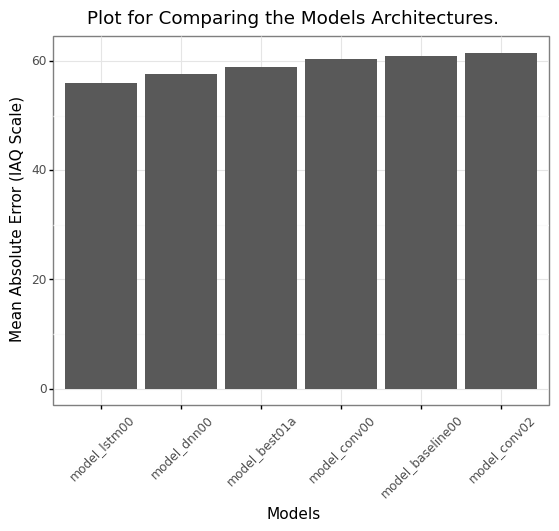
\includegraphics[scale=0.45]{image01.png}
    \caption{We tested 10 different neural network types, including: Dense
    (Perceptron), LSTM, Convolutional, Recursive networks and combinations
    of them.}
    \label{fig1}
\end{figure}

\begin{table}[!ht]
    \centering
    \begin{tabular}{|l|l|l|l|l|l|l|l|l|l|l|}
    \hline
        Model & Time & Epochs & W. Sz. & Stride & Samp. Rt. & MSE & MAE & Re Sample \\ \hline
        lstm00 & 47.62 & 11 & 30 & 2 & 2 & 0.0249 & 55.97 & 10 Min \\ \hline
        dnn00 & 29.58 & 14 & 15 & 1 & 2 & 0.0309 & 57.58 & 10 Min \\ \hline
        best01a & 890.75 & 28 & 15 & 1 & 2 & 0.0244 & 59.03 &  05 Min \\ \hline
        conv00 & 79.88 & 14 & 15 & 1 & 2 & 0.0301 & 60.34 & 10 Min \\ \hline
        baseline00 & 24.97 & 14 & 15 & 1 & 2 & 0.0325 & 60.90 & 10 Min \\ \hline
        conv02 & 799.29 & 28 & 15 & 1 & 2 & 0.0207 & 61.58 & 05 Min \\ \hline
    \end{tabular}
    \caption{Comparison of different architectures. 
    Stride and for Sample Rate were handled as hyperparameters
    of Tensorflow time-series window generator \cite{kerasWeather,tfTimeseries}. 
    W. Sz. means Window size in days.}
\end{table}


\begin{figure}
    \centering
    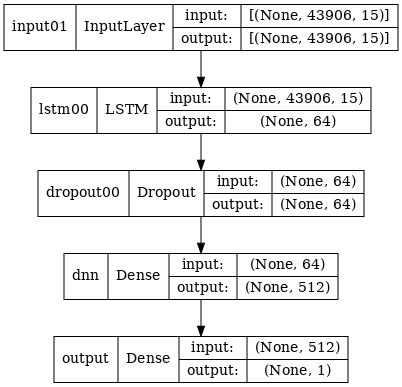
\includegraphics[scale=0.45]{image02.png}
    \caption{lstm00 model is a 3 layer combining LSTM, dropout and dense layers in the following fashion. LSTM layer was implemented as 64 LSTM neurons, a second dropout layer with a rate of 0.5 to avoid overfitting and lastly a 512 perceptron RELU activated layer. This model has a total of 576 neurons. }
    \label{fig2}
\end{figure}


    \hypertarget{performance-of-the-models.}{%
\subsubsection{Performance of the
Models.}\label{performance-of-the-models.}}

These architectures were tuned with different time-series hyperparamters
to check for consistency of performance on our architectures with our
data and to optimize our computational budget. We found that the
re sampling size of our dataset, i.e.: instead of processing all our
sensor records every 3 seconds it is useful to get the means of these
records every 1, 2 ad 5 minutes. 


    Our budget did not allow us to fully test the performance of the 1 minutes
re sampling data, as it was very expensive. And the 2 and 5 minutes re samples
are comparable performance-wise. Then we tested and even larger re sample
of 10 minutes with great results.


    \hypertarget{conclusions}{%
    \section{Conclusions.}\label{conclusions}}

In this paper, we faced the problem of not having accurate and
up-to-date information on air quality living in a city with pollution
problems. This lack of information led us to ask ourselves what we could
contribute as Data Scientists, so we have developed some air quality
prediction models based on neural network systems. We proposed a variety
of methods with both the scopes of concerned: to perform multi-layer
perceptron models for predicting IAQ concentration in an indoor sensor
and to compare the performances between different time-windows and a
baseline model.

Data for model classification training was collected using an IAQ Bosch
monitoring system. In addition to information from our sensor, we
collated data with information from external sources that included
particulates such as carbon dioxide, carbon monoxide, ozone, nitrogen
dioxide, oxygen, volatile organic compounds, and particulates,
temperature, and humidity. Based on the results of the network models,
LSTM model was the best with a MAE of 55.97, nevertheless,all our models 
presented a similar performance.

In general, it can be concluded that the system delivered a high
classification rate based on LSTM. We attribute this success to the
appropriate use of time windows and the advantage that Vertex gave us to
be able to perform tests with large amounts of data.

The developed models can help environmental agencies and governments
monitor air pollution levels more efficiently. Moreover, the model can
help to correct missing information in order to protect the health of
the citizens who are inhabiting in metropolitan areas.

With high hopes, in the future we would like to work, at least, with
data from a full year, to deal with seasonality and its effects on the
measurement. We will probably extend this work to a project where the
effects of air quality in a pandemic environment are considered.

%    \hypertarget{appendices.}{%
%\subsection{Appendices.}\label{appendices.}}


\begin{thebibliography}{8}
    
    \bibitem{abdullah}
    Abdullah, A., Raja S., Thulasyammal R.,  Mohsen M, Ibrahim A.: An Optimized Artificial Neural Network Model Using Genetic Algorithm for Prediction of Traffic Emission Concentrations. International Journal of Advanced Computer Science and Applications, vol. 12. The Science and Information Organization. \doi{10.14569/IJACSA.2021.0120693}. (2021)
    
    \bibitem{cakir}
    Cakir, S., Moro S.: Evaluating the Performance of Ann in Predicting the Concentrations of Ambient Air Pollutants in Nicosia. Atmospheric Pollution Research, Vol. 11, Issue 12, pp. 2327-2334. \doi{10.1016/j.apr.2020.06.011}. (2020)
    
    \bibitem{ghazali}
    Ghazali S., Lokman H.: Air Quality Prediction Using Artificial Neural Network. Universiti Tun Hussein Onn Malaysia. The International Conference on Civil and Environmental Engineering Sustainability. \url{http://eprints.uthm.edu.my/2528/1/Air_Quality_Prediction_Using_Artificial_Neural_Network.pdf}. (2012)
    
    % \bibitem{haddad}
    % Haddad R., Abebe M., Yehudah R., David H., Noam S.: Predicting Odor Pleasantness with an Electronic Nose. PLoS Computational Biology \textbf{6}(4). (2010)
    
    \bibitem{patni}
    Patni J., Sharma H.: Air Quality Prediction using Artificial Neural Networks. International Conference on Automation, Computational and Technology Management. \doi{10.1109/icactm.2019.8776774.} (2019)
    
    % \bibitem{muhammad}
    % Nur H., Muhammad H., MohdTalib L., Suhartono: Forecasting of Air Pollution Index with Artificial Neural Network. Jurnal Teknologi. \textbf{63}(2). (2013)
    
    \bibitem{saad}
    Saad S., Andrew A, Shakaff A., Saad A., Yuzof A., Zakaria A.: Classifying Sources Influencing Indoor Air Quality (IAQ) Using Artificial Neural Network (ANN). Sensors. \textbf{15}(5). (2015)
    
    \bibitem{bekkar}
    Bekkar, A., Hssina, B., Douzi, S. et al. Air-pollution prediction in smart city, deep learning approach. Journal of Big Data \textbf{8}(161). 
    \doi{10.1186/s40537-021-00548-1}
    (2021)
    
    \bibitem{sotomayor}
    Sotomayor-Olmedo, A., Aceves-Fernández, M., Gorrostieta-Hurtado, E., Pedraza-Ortega, C., Ramos-Arreguín, J., and Vargas-Soto, J.: Forecast Urban Air Pollution in Mexico City by Using Support Vector Machines: A Kernel Performance Approach, International Journal of Intelligence Science, \textbf{3}(3), pp. 126-135. \doi{10.4236/ijis.2013.33014}.
    (2013)
    
    \bibitem{ramosibarra}
    Ramos-Ibarra, E., Silva, E.: Trend estimation and forecasting of atmospheric pollutants in the Mexico City Metropolitan Area through a non-parametric perspective,
    Atmósfera: \textbf{33}(4), p.401-420. 
    \doi{10.20937/ATM.52757}.
    (2020)
    
    \bibitem{bing}
    Bing, G., Ordieres–Meré, J., and Cabrera, C.:
    Prediction models for ozone in metropolitan area of Mexico City based on artificial intelligence techniques. 
    International Journal of Information and Decision Sciences, \textbf{7}(2), 115-139.
    \doi{10.1504/IJIDS.2015.068756}
    (2015)
    
    \bibitem{singh}
    S. K. Singh, R. Yang, A. Behjat, R. Rai, S. Chowdhury and I. Matei, 
    PI-LSTM: Physics-Infused Long Short-Term Memory Network.
    18th IEEE International Conference On Machine Learning And Applications (ICMLA), 2019, pp. 34-41, \doi{10.1109/ICMLA.2019.00015}.
    (2019)
    
    \bibitem{airpollution}
    Kim, Y., Knowles, S., Manley, J., Radoias, V. Long-run 
    health consequences of air pollution: Evidence from 
    Indonesia's forest fires of 1997. Economics \& Human Biology
    \textbf{26}, pp. 186-198, 
    \doi{10.1016/j.ehb.2017.03.006}.
    (2017)
    
    \bibitem{nom156}
    NORMA Oficial Mexicana NOM-156-SEMARNAT-2012, 
    Establecimiento y operación de sistemas de monitoreo
    de la calidad del aire. \S 10.4.2,
    pp 8, 14. (2012) 
    \url{https://sinaica.inecc.gob.mx/archivo/noms/NOM-156-SEMARNAT-2012.pdf}.
    Last accessed 20 Feb 2022.
    

    % \bibitem{sensortec1}
    % Bosch Sensortec Community \textbar\ How do I convert BME 680
    % gas resistance to IAQ?, \url{https://community.bosch-sensortec.com/t5/Question-and-answers/How-do-I-convert-BME680-gas-resistance-to-IAQ/qaq-p/9050/comment-id/94#M94}. 
    % Last accessed Oct 3, 2021.
    
    % \bibitem{sensortec2}
    % Bosch SensorTec Community \textbar\ Solution to IAQ accuracy  definition,
    % \url{https://community.bosch-sensortec.com/t5/MEMS-sensors-forum/BME680-IAQ-accuracy-definition/m-p/5931/highlight/true#M10}. 
    % Last accessed 3 Oct, 2021.
    
    % \bibitem{githubMancuso}
    % GitHub \textbar\ Daniel Mancuso: Código fuente de OhmTech-io/uThingVOC Src/main.c ,
    % \url{https://github.com/ohmtech-io/uThingVOC/blob/f345fdbef6a4fd0da77289b436e3c478706572a2/Src/main.c#L139}.
    % Last accessed 3 Oct 2021.
    
    \bibitem{kerasWeather}
    Keras / Code examples / Timeseries / Timeseries forecasting for weather prediction,
    \url{https://keras.io/examples/timeseries/timeseries_weather_forecasting/}.
    Last accessed 3 Oct 2021.
    
    \bibitem{tfTimeseries}
    Tensorflow: Tutorial on Time series forecasting Time series forecasting,
    \url{https://www.tensorflow.org/tutorials/structured_data/time_series}.
    Last accessed 3 Oct 2021.
    
    \bibitem{bme680}
    Bosch BME680 Datasheet, 
    \url{https://www.bosch-sensortec.com/media/boschsensortec/downloads/datasheets/bst-bme680-ds001.pdf}.
    Last accessed 3 Oct 2021.
    
    \bibitem{mancuso}
    Mancuso, D. Indoor Air Quality Monitor \textbar\ Hackster.io,
    \url{https://www.hackster.io/damancuso/indoor-air-quality-monitor-b181e9}.
    Last accessed 3 Oct 2021.
    
    \bibitem{sedema}
    Dirección de Monitoreo Atmosférico de la Secretaría del Medio Ambiente del Gobierno de la Ciudad de México,
    \url{http://www.aire.cdmx.gob.mx/}.
    Last accessed 3 Oct 2021.
    
    \bibitem{openweather}
    OpenWeatherMap: History weather bulk for Camarones (19.48,-99.18) from January 01, 1979 to September 27, 2021.
    \url{https://openweathermap.org/history-bulk}
    Last accessed 27 Sep, 2021.
    
    \bibitem{sinaica}
    Sistema Nacional de Información de la Calidad del Aire del Gobierno Federal México]
    \url{https://sinaica.inecc.gob.mx/}.
    Last accessed 3 Oct 2021.
    
    \bibitem{googlecolab}
    Google AI Blog: Doing Data Science with coLaboratory.
    \url{https://ai.googleblog.com/2014/08/doing-data-science-with-colaboratory.html}.
    Last accessed 21 Feb 2022.
    
    \bibitem{vertexai}
    Google Cloud launches Vertex AI, unified 
    platform for MLOps \textbar\ Google Cloud Blog.
    \url{https://cloud.google.com/blog/products/ai-machine-learning/google-cloud-launches-vertex-ai-unified-platform-for-mlops}
    Last accessed 21 Feb 2022.
    % \bibitem{ref_article1}
    % Author, F.: Article title. Journal \textbf{2}(5), 99--110 (2016)
    
    % \bibitem{ref_proc1}
    % Author, A.-B.: Contribution title. In: 9th International Proceedings
    % on Proceedings, pp. 1--2. Publisher, Location (2010)
    
    % \bibitem{ref_url1}
    % LNCS Homepage, \url{http://www.springer.com/lncs}. Last accessed 4
    % Oct 2017
    
    \bibitem{abadi}
    Abadi, M., Agarwal, A., Barham, P., et al: TensorFlow: Large-scale machine learning on heterogeneous systems. 
    \url{https://arxiv.org/abs/1603.04467}. 
    (2015)
    
    %\bibitem{saadi}
    %Saadi S., et al. Development of indoor environmental index: Air quality index and thermal comfort index. 
    %\doi{10.1063/1.4975276}.
    %2017)
    
    %\bibitem{mckinney}. 
    %McKinney, W. 
    %Data structures for statistical computing in Python: SciPy 2010 Conference.
    %\url{https://conference.scipy.org/proceedings/scipy2010/pdfs/mckinney.pdf}. (2010)
    
    %\bibitem{matplotlib}
    %Hunter, J. Matplotlib: A 2D Graphics Environment. 
    %\doi{10.5281/zenodo.592536/zenodo.592536}
    %(2007)
    
    %\bibitem{paco}
    %Román-Rangel, F. Notes and code for the Deep Learning course: MSc Data Science Program. 
    %Instituto Tecnológico Autónomo de México, Mexico City. (2020)
\end{thebibliography}

\end{document}
